\subsubsection*{Parte B}

\begin{center}
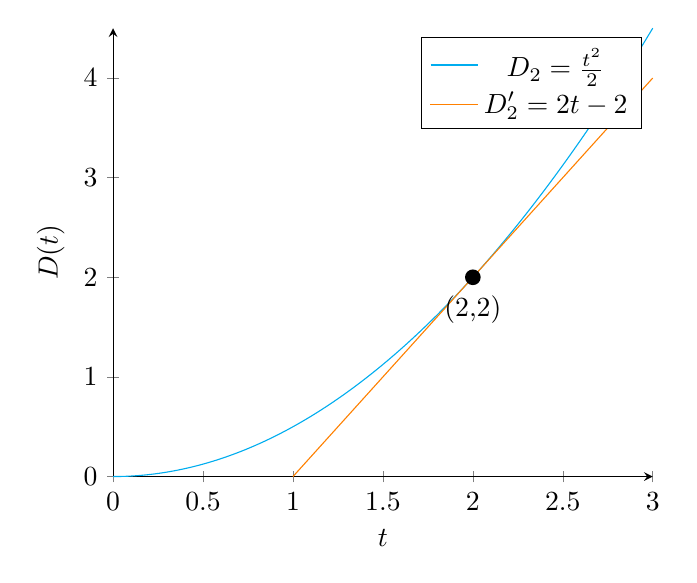
\begin{tikzpicture}
\begin{axis}[
    axis lines = left,
    xlabel = \(t\),
    ylabel = {\(D(t)\)},
    clip = false,
]

% D_2
\addplot[
    domain=0:3,
    samples=200,
    color=cyan,
]
{x*x/2};
\addlegendentry{\(D_2=\frac{t^2}{2}\)}

% Derivada que pasa por 2
\addplot[
    domain=1:3,
    samples=200,
    color=orange,
]
{2*x-2};
\addlegendentry{\(D'_2=2t-2\)}

\node[label={270:{(2,2)}},circle,fill,inner sep=2pt] at (axis cs:2,2) {};

\end{axis}
\end{tikzpicture}
\end{center}

Para obtener la función que describe a la recta tangente a la función en el punto $(2, 2)$ expresamos este punto en la notación punto-pendiente, incluyendo como pendiente al valor devuelto por la derivada de $D_2$, que en ese punto es 2. Entonces:

\begin{align*}
    y-2 &= 2(x-2)\\
    y &= 2x - 4 + 2\\
    y &= 2x - 2
\end{align*}

Por otra parte, para obtener la función que describe la recta secante correspondiente al intervalo $[1,5; 2]$, calculamos en primer lugar su pendiente:

\begin{align*}
    m &= \frac{D_{2(2)} - D_{2(1,5)}}{2 - 1,5}\\
    m &= \frac{2 - 9/8}{2 - 1,5}\\
    m &= \frac{7}{4}
\end{align*}

Con la expresión de la pendiente, tomamos uno de los puntos por el cual deseamos que cruce, en este caso puede ser $(2, 2)$, y planteamos la función en notación punto-pendiente:

\begin{align*}
    y-2 &= \frac{7}{4}(x-2)\\
    y &= \frac{7}{4}x - \frac{7}{2} + 2\\
    y &= \frac{7}{4}x - \frac{3}{2}
\end{align*}

Con la expresión $y = \frac{7}{4}x - \frac{3}{2}$, podemos representar la secante.

\begin{center}
\begin{tikzpicture}
\begin{axis}[
    axis lines = left,
    xlabel = \(t\),
    ylabel = {\(D(t)\)},
    clip = false,
]

% D_2
\addplot[
    domain=1:3,
    samples=200,
    color=cyan,
]
{x*x/2};
\addlegendentry{\(D_2=\frac{t^2}{2}\)}

% Secante que pasa por 2
\addplot[
    domain=1.5:2,
    samples=200,
    color=magenta,
]
{7/4*x-3/2};
\addlegendentry{\(S=\frac{7}{4}t - \frac{3}{2}\)}

\node[label={270:{(2,2)}},circle,fill,inner sep=2pt] at (axis cs:2,2) {};
\node[label={270:{(1,5,9/8)}},circle,fill,inner sep=2pt] at (axis cs:1.5,1.125) {};
\end{axis}
\end{tikzpicture}
\end{center}

\begin{center}
\begin{tabular}{ c c c c c c c c c c c c }
    t & 1,5 & 1,9 & 1,99 & 1,999 & 1,9999 & 2 & 2,0001 & 2,001 & 2,01 & 2,1 & 2,5\\
	\hline \\
    $g_{(t)} = \frac{t^2}{2}$ & 1.125 & 1.805 & 1.98 & 1.998 & 1.9998 & 2 & 2.0002 & 2.002 & 2.02 & 2.205 & 3.125 \\
    \vspace{10pt} \\
    $\frac{g_(t) - g_(2)}{t - 2}$ & 1.75 & 1.95 & 2 & 2 & 2 & 2 & 2 & 2 & 2 & 2.05 & 2.25\\
    \vspace{10pt} \\
    \hline
\end{tabular}
\end{center}

Como puede observarse tanto en las gráficas como en la tabla construida, a medida que los extremos de la recta secante se aproximan, el valor de su pendiente tiende al valor de la derivada en dicho punto.